\subsection{Architecture}
This particular section describes the architecture details of the centralized Secure Package service. The frontend application was developed in Angular 5. It is connected to a PHP backend, with a MySQL database for storage of data, via an API. During the development process, the application was hosted locally, using various tools, which are described in Section \ref{section:tools}. Details, regarding the workflow and the implementation process itself are described in Section \ref{section:development}.

\subsubsection{Abstract data structures} \label{section:datastructures}
In order to provide intended functionality of the system, several abstract data structures were defined to digitally represent various features of the application and its semantics. It is important to note that some of those structures were stored across several database tables (detailed description of that is provided in \ref{section:backend}), as some of them consist of a number of substructures which needed to be differentiated in order to organize data in more efficient manner.

\paragraph{User account} 
This structure represents a user account and its semantics. A user account is required in order to access the majority of service's functionality. User accounts are configured with the private and public keys, a password, as well as personal information, such as full name and address (needed for logistics purposes). 160-bit account identifiers are derived from public keys, using the same principal, as in Ethereum account generation. Private information (such as personal details) are to be protected from outsiders and available only to the logistics company during the logistics process.

\paragraph{Clerk account}
Clerk accounts are required to perform clerk operations, which are related to conflict resolving. Clerk administrators are not granted access to personal information, unless the conflict request was initiated. This type of account is configured with a unique username and a password.

\paragraph{Agreement}
By far the most extensive abstract structure in the context of the centralized Secure Package system is the agreement structure. It encapsulates the semantics and parameters of the whole process of merchandise transfer from the point of advertisement publication by the seller to the termination of the transfer process. Agreement itself contains an item, a selection of terms, as well as some other parameters. One of the additional and most defining parameters of the agreement is its state, which dynamically changes according to the agreement related events (that topic is brought up in greater detail in Section \ref{section:statesofcontract}).

\paragraph{Item}
Details about the item itself, such as the title, images and the description, compile the abstract data structure which represents items. This structure can be seen as a substructure of the agreement.

\paragraph{Terms}
Terms data structure can be interpreted as a set of rules for the agreement. That, in its turn, implies that it is a substructure of the agreement. Terms consist out of sensor configurations, as well as proposed item price, identification numbers, among other things. Agreement terms are also configured with a status parameter. That parameter is changed depending on whether the terms were accepted, or declined by the agreement initiator (the seller). 

\paragraph{Event}
Event structure defines events, which are related to the agreements. Events are mainly used for altering states of the agreements. The structure contains event details, which are necessary in order to correctly alter states (that topic is brought up in greater detail in Section \ref{section:statesofcontract}).

\paragraph{Logistics process}
General details about the logistics process, such as the identification number, sensor selection and related agreement, are encapsulated in that data structure. That structure is mainly used for interaction with logistics transport simulator, which is described in Section \ref{section:simulation}.

\paragraph{Sensor}
Sensor structure defines the semantics of sensors, as well as their threshold configuration. It acts as a substructure of the logistics process structure. It is also used in large extent for interaction with the simulator module.

\paragraph{Conflict}
Conflict data structure defines clerk resolving process for agreements, that at some point generated a conflict request. Such request is automatically generated in case of seller declining the potential return.

\subsubsection{Frontend} \label{section:frontend}
A good and user-friendly frontend is necessary in order to provide good user experience in a web application. The frontend was implemented mainly in TypeScript and HTML, using Angular, which is a TypeScript-based open-source frontend web application platform \citep{angular}. During the development, debugging and testing process, the frontend application was deployed, using a local Webpack Dev Server (WDS).

\paragraph{Functionality}
The goal of the frontend was to present application in form of an online web marketplace. The frontend was to provide responsive interface for posting new advertisements, as well as browsing the existing ones was implemented, along with functionality of performing actions, such as making proposals and managing own advertisements. Various functional modules of the application were implemented using pop-up modals. Users were also introduced with the ability to change some of the account information from the frontend. 

One of the things, which was kept in mind during the development process of the frontend, was to differentiate its modules, according to the functionality, in order to reduce coupling and increase cohesion. That was also one of the main choices for choosing Angular library for implementation (more detailed discussion about the reasons behind that statement is provided in the next paragraph).

\paragraph{Components}
Angular applications are typically built, using components, which can be seen as modules, or building blocks of a software. That approach is very desirable, as it allows the code being very organized, according to functional properties. It results in reduced coupling and provides high cohesion, which is very desirable, as it improves system's modifiability and reusability, while making code more comprehensible. The frontend application was divided into the following Angular components:

\begin{itemize}
\item \texttt{AgreementComponent} - Accessible only by the buyer and the seller for detailed information about a particular active agreement and its logistics processes (with sensor visualization). Delivery and return feedback functionality is accessed in that particular component as well. 

\item \texttt{ClerkComponent} - Used by clerk administrators to browse and resolve conflict requests. Can only be accessed by logging in with a special clerk account.

\item \texttt{ExplorerComponent} - Has similar functionalities to block explorer applications for blockchain networks. Users are able to search for specific identifiers (addresses) in order to find detailed information about them. In order to increase the system's transparency, this component is accessible to anyone, without having to log in to the application.

\item \texttt{ItemComponent} - Displays detailed information about the item (title, picture, description, initial terms), as well as all current proposals by potential buyers. Logged in users may propose terms in this component.

\item \texttt{ItemBrowserComponent} - Displays the list of advertisements, which have not yet been locked. Detailed information about a particular item can be browsed by clicking the agreement, which would redirect the user to \texttt{ItemComponent}.

\item \texttt{ItemManagerComponent} - Accessible only by logged in users and is used for agreement and proposal management. Acceptance and denial of proposed terms is handled through that component, as well as overall information about user's proposals, items and historical agreements.

\item \texttt{LoginComponent} - Start page of the application. Used to generate new accounts and log in with the existing ones.

\item \texttt{NewItemComponent} - Provides the functionality of creating new agreement, as well as defining the related item and its initial terms. Accessible only by the logged in users.

\item \texttt{AppComponent} - Provides top and bottom navigation bars and routing, according to navigation bar buttons.
\end{itemize}

Each component is defined by a template HTML document, as well as a TypeScript file, which define its semantics and manages the data.

\paragraph{Design and appearance}
In order to improve visual aspects of the application, some CSS stylesheets were implemented. Majority of the styling was done, using the front-end component library called Bootstrap. Some of the CSS classes were overwritten in local CSS files, in order to tailor specific components of the application according to web interface's visual appeal.

\paragraph{Communication with the backend}
All of the communication with the backend was done using the \texttt{ApiService}, as it would provide some benefits, which were described in the theoretical analysis in Section \ref{section:reuse}. One of its tasks is to send and receive HTTP calls to and from the designated server address. The service parses the received HTTP response payload data into JSON objects, which can later be used by the component, that initiated the HTTP call, to manipulate its internal variables etc. The process of API call functionality is visualized in the data flow chart in Figure \ref{fig:dataflow}.

\subsubsection{Backend} \label{section:backend}

\paragraph{Database}
When deciding what database model to use for a system's backend, there are many different choices to consider. It is important to make that decision based on the specific features and demands of the application in question. Based on that reasoning principal, MySQL relational database was chosen, as it was considered to suit the requirements of a merchandise trading and transport platform application rather well. It has numerous advantages that Secure Package application can potentially benefit from, such as great levels of security, on-demand scalability, high availability and comprehensive transaction support, among other features \citep{mysqladvantages}. Another reason for choosing a relational database is that majority of the abstract data structures from Section \ref{section:datastructures} have strong connections to eachother (such as substructures and superstructures), which could easily be represented with foreign keys. Nearly all instances of structures are to be configured with unique identifiers, thus making them perfect primary keys.

In order to come up with a suitable database structure, the abstract structures from Section \ref{section:datastructures} were carefully analyzed. For example, it is obvious that many structures has references to the agreements structure. Those references are represented by foreign keys. Based on that analysis, the following database tables were proposed:

\begin{itemize}
\item \texttt{agreements} - Stores instances of agreements, their corresponding parameters and semantics. Has (1:1) foreign key references to \texttt{accounts} to represent buyer and seller accounts. Primary key of this table is a 160-bit agreement identifier.

\item \texttt{agreement\_events} - Stores instances of events and their corresponding parameters. Each event instance is related to exactly one agreement (agreements can have multiple events). Therefore the table is related to \texttt{agreements} table in (n:1) manner with that relation being represented by a foreign key. Primary key of this table is represented by unique 160-bit event identifiers.

\item \texttt{terms} - Stores instances of the terms structure, along with their semantics and corresponding parameters. Has a (n:1) foreign key reference to \texttt{agreements}, as many terms can be proposed to a single agreement. Primary key of this table is represented by unique 160-bit terms identifiers.

\item \texttt{items} - Stores parameters of the item structure. Has a (1:1) foreign key reference to \texttt{agreements}, as each agreement can only be associated with exactly one item and vice versa. Primary key of this table is represented by unique 160-bit item identifiers.

\item \texttt{images} - Stores images of an item, which is a part of the item structure. There is support for multiple images of a single item, therefore the table has a (n:1) foreign key relation to the \texttt{items} table. Primary key of this table is represented by unique 160-bit image identifiers.

\item \texttt{accounts} - Stores instances of user accounts, along with the corresponding parameters. Primary key of this table is represented by unique 160-bit user account identifiers, which are derived from the corresponding public keys (stored in the same table).

\item \texttt{clerk\_accounts} - Stores instances of clerk user accounts, along with the corresponding parameters. Primary key of this table is represented by unique clerk usernames.

\item \texttt{clerk\_actions} - Stores instances of conflict structures and their corresponding parameters. Has a (1:1) relation with the \texttt{agreements} table, with the primary key of this table being represented by unique 160-bit agreement identifier, which also acts as a foreign key. Has also a (n:1) relation to the \texttt{clerk\_accounts} table.

\item \texttt{logistics\_simulation} - Stores instances of logistics process data structures, as well as their corresponding parameters and semantics. Has a (n:1) relation with the \texttt{agreements} table in form of a foreign key. Primary key of this table is represented by unique parcel identifiers.

\item \texttt{sensors} - Stores instances of sensor structures. Has a (1:1) foreign key relation with the \texttt{logistics\_simulation} as each sensor can only be associated with exactly one logistics process. Primary key of this table is represented by unique 160-bit sensor identifiers. 

\item \texttt{sensor\_data} - Stores sensor output data, which is a part of sensor structure. Each sensor output will produce a row in the table. Has (n:1) relation with the \texttt{sensors} table in form of a foreign key. Does not possess any primary key.

\item \texttt{gps\_data} - Stores gps sensor output data, which is a part of sensor structure. Has (1:1) relation with the \texttt{sensors} table in form of a foreign key. Does not possess any primary key.
\end{itemize}

In order to visualize the database structure, a database schema was crated, using the reverse engineering tool, integrated into MySQL Workbench software, which was used for database generation and management purposes. The schema is displayed in Figure \ref{fig:databaseschema} and it consists out of two different modules. The \texttt{Secure Package} module is responsible for maintaining Secure Package application data, while the \texttt{Logistics Simulation} module maintains logistics process data and is mainly used for interaction with the logistics process simulation, which is described in Section \ref{section:simulation}.

\begin{figure}[H]
\centering
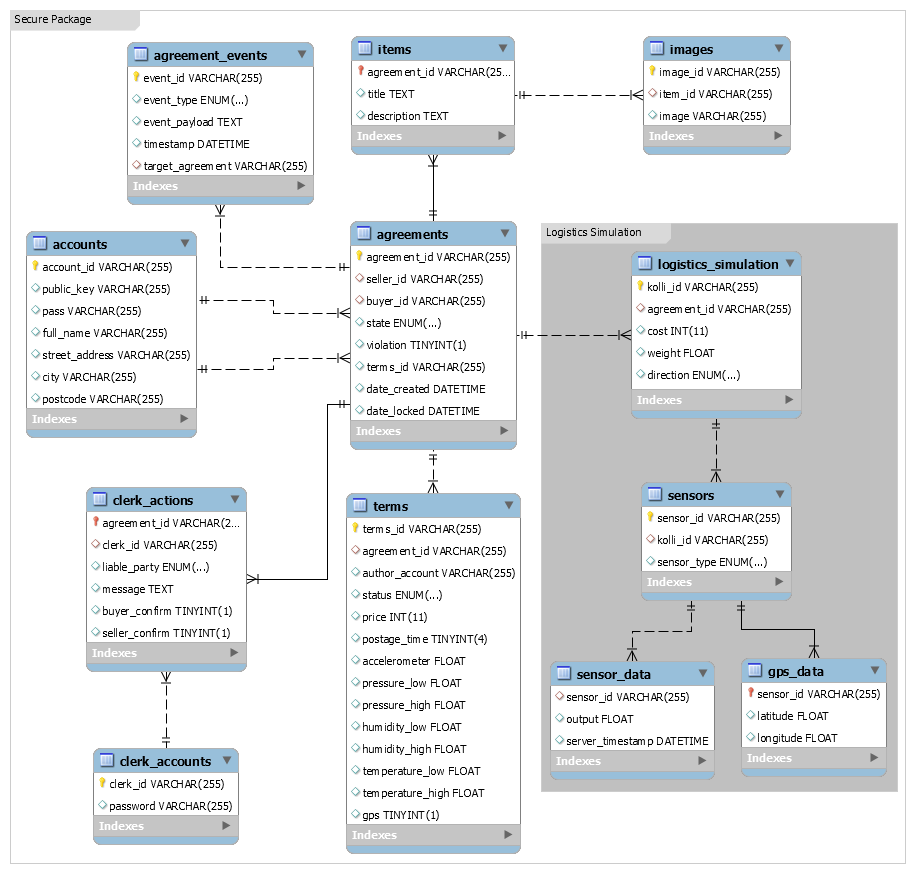
\includegraphics[scale=0.4]{images/database.png}
\caption{Database schema of the centralized Secure Package system.}
\label{fig:databaseschema}
\end{figure}

\paragraph{Application programming interface (API)}
As was mentioned in \ref{section:reuse}, implementation of an application programming interface (API) generally improves code's reusability and modifiability, while making it more comprehensible to other programmers. Therefore, the approach, similar to Facade API pattern was used during the implementation process. The API was developed as a part of the backend. It handles incoming HTTP calls from the frontend's \texttt{ApiService} (more detailed description is provided in Section \ref{section:frontend}) and performs database operations, depending on the \texttt{action} field of the HTTP call. The code, which is related to handling is located in \texttt{http\_handler} file. The \texttt{http\_handler} in its turn makes calls to function inside the \texttt{function\_library} module, which then performs database operations. 

In vast majority of cases, the API is required to send some data back to the application, which is achieved through encoding response data into JSON format before echoing it back to the frontend. This functionality is also implemented within the \texttt{http\_handler}.

Detailed schematics of API communication can be seen in the data flow diagram in Figure \ref{fig:dataflow}.

\begin{figure}[H]
\centering
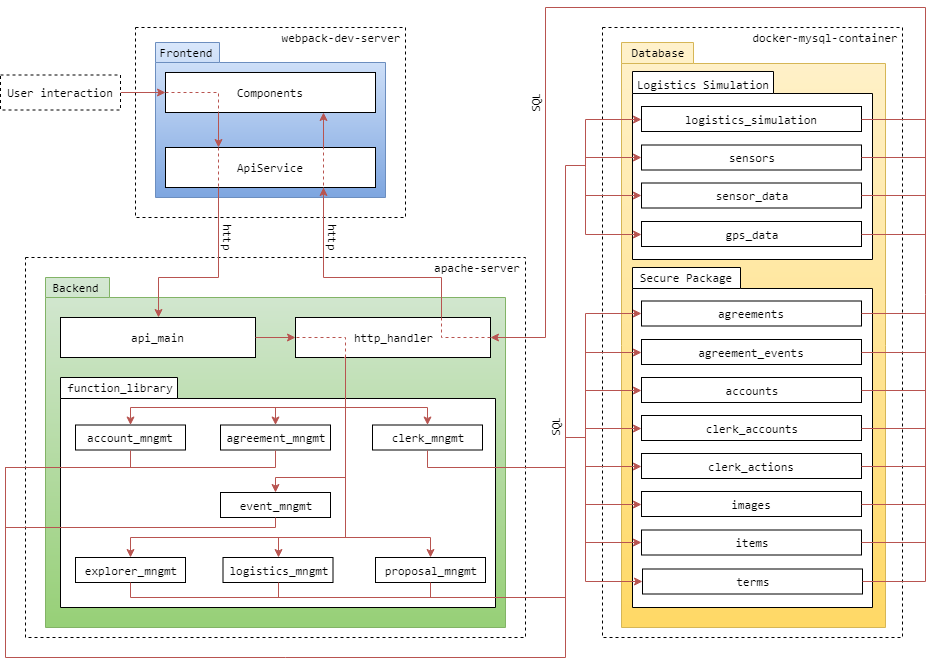
\includegraphics[scale=0.49]{images/dataflow.png}
\caption{Data flow diagram of the API calls.}
\label{fig:dataflow}
\end{figure}

The API, as well as all of the server-side code in the \texttt{function\_library} was written in PHP and was deployed on an Apache MySQL server during the development process. The server itself was hosted locally, using a software, called XAMPP. 

\subsubsection{Semantics of the agreement} \label{section:statesofcontract}
As was mentioned in Section \ref{section:datastructures}, the whole mechanism of merchandise transfer from the point of publication of advertisement to seller, receiving the goods, is encapsulated in an abstract structure, called agreement. The agreements are stored in a database and correspond to a single row in table \texttt{agreements}. The field, which is responsible for the current status of the agreement is called \texttt{agreements.state}, which acts like an enumerated type with following predefined options: \texttt{Created}, \texttt{Locked}, \texttt{Transit}, \texttt{Deliv}, \texttt{Return}, \texttt{Returned}, \texttt{Clerk} and \texttt{Inactive}. 

Boolean parameters, that represent sensor threshold violations, are stored in the database field \texttt{agreements.violated}. This parameter is used along with with the parameter, stored in \texttt{agreements.state}, to represent condition of the agreement.

\paragraph{Deterministic finite automaton}

In order to visually represent the semantics of state transitions and event occurrence in a given agreement, a special type of Turing Machine was constructed, called a deterministic finite automaton (DFA) \citep{dfa}. A deterministic finite automaton, in general, is a 5-tuple $(Q, \Sigma, \delta, q_{0}, F)$, where:

\begin{itemize}
\item $Q$ is a finite set of states.
\item $\Sigma$ is an alphabet called the input alphabet.
\item $\delta: Q \times \Sigma \rightarrow Q$ is the transition function.
\item $q_0 \in Q$ is the starting state.
\item $F \subseteq Q$ is the set of accepting states.
\end{itemize}

Using the definition above, a DFA, denoted as $M$, was constructed. The set of states $Q$ consists out of all possible values of \texttt{agreements.state} parameter. A drawback which is associated with DFAs is that they do not possess memory \citep{alexisdfa}. Thus, some of the options in \texttt{agreements.state} are duplicated, depending, whether the \texttt{agreements.violated} boolean parameter is \texttt{True} or \texttt{False}. The set of states $Q$ is listed in Table \ref{tab:states}. The transitions are triggered by a range of agreement-related events, which construct the input alphabet $\Sigma$. These events are also listed in Table \ref{tab:states}.


The relation between members of $Q$ is established by the occurrence of the selection of events, defined in $\Sigma$, using the transfer function  $\delta: Q \times \Sigma \rightarrow Q$. In context of the Secure Package system, $\delta$ takes following shape:
\bigskip

\begin{table}[H]
\begin{center}
\begin{tabular}{ c|c c c c c c c c c c c c c c c c} 
 $\delta$ & $e_{p}$ & $e_{a}$ & $e_{d}$ & $e_{sp}$ & $e_{bt}$ & $e_{st}$ & $e_{v}$ & $e_{by}$ & $e_{sy}$ & $e_{bn}$ & $e_{sn}$ & $e_{bf}$ & $e_{sf}$ & $e_{bc}$ & $e_{sc}$ & $e_{c}$\\ 
 \hline
$\boxed{q_{s}}$ & $q_{s}$ & $q_{l}$ & $q_{s}$ & - & - & - & - & - & - & - & - & - & - & $q_{s}$ & \underline{$q_{a}$} & -\\ 
 $q_{l}$ & - & - & - & $q_{t}$ & - & - & - & - & - & - & - & - & - & \underline{$q_{a}$} & \underline{$q_{a}$} & -  \\ 
 $q_{t}$ & - & - & - & - & $q_{d}$ & - & $q_{tv}$ & - & - & - & - & - & - & - & - & -  \\
 $q_{tv}$ & - & - & - & - & $q_{dv}$ & - & $q_{tv}$ & - & - & - & - & - & - & - & - & -  \\ 
 $q_{d}$ & - & - & - & - & - & - & - & \underline{$q_{c}$} & $q_{r}$ & - & - & - & $q_{c}$ & - & - & -  \\
 $q_{dv}$ & - & - & - & - & - & - & - & \underline{$q_{c}$} & $q_{rv}$ & - & - & - & $q_{c}$ & - & - & -  \\  
 $q_{r}$ & - & - & - & - & - & $q_{b}$ & $q_{rv}$ & - & - & - & - & - & - & - & - & -  \\ 
 $q_{rv}$ & - & - & - & - & - & $q_{bv}$ & $q_{rv}$ & - & - & - & - & - & - & - & - & -  \\ 
 $q_{b}$ & - & - & - & - & - & - & - & - & \underline{$q_{a}$} & - & $q_{j}$ & - & \underline{$q_{a}$} & - & - & -  \\ 
 $q_{bv}$ & - & - & - & - & - & - & - & - & \underline{$q_{a}$} & - & $q_{jv}$ & - & \underline{$q_{a}$} & - & - & - \\ 
 $q_{j}$ & - & - & - & - & - & - & - & - & - & - & - & - & - & - & - & \underline{$q_{a}$}  \\ 
 $q_{jv}$ & - & - & - & - & - & - & - & - & - & - & - & - & - & - & - & \underline{$q_{a}$}  \\ 
 \underline{$q_{a}$} & - & - & - & - & - & - & - & - & - & - & - & - & - & - & - & -  \\ 
 \underline{$q_{c}$} & - & - & - & - & - & - & - & - & - & - & - & - & - & - & - & - \\ 
 \end{tabular}
 \caption {The table, which defines the transition function $\delta: Q \times \Sigma \rightarrow Q$. }
 \label{tab:deltafunction}
\end{center}
\end{table}

\begin{table}[H]
\begin{tabular}{| c | l |}
\hline
\textbf{State} $\forall q \in Q$& \textbf{Description}\\
\hline
{\tiny CREATED} ($q_{s}$)&  Contract is initiated. \\
{\tiny LOCKED} ($q_{l}$)&  Terms have been accepted by the seller.\\
{\tiny TRANSIT} ($q_{t}$)&  The item is being transported by the logistics company. \\
{\tiny TRANSIT$_\mathrm{V}$} ($q_{tv}$)&  Sensors have detected violation of the threshold during the transfer.\\
{\tiny DELIV} ($q_{dv}$)&  Item is received by the buyer (threshold was not violated during the \\ & transfer), money is transferred to the third party. \\
{\tiny DELIV$_\mathrm{V}$} ($q_{dv}$)&  Item is received by the buyer (threshold was violated during the \\ & transfer), money is transferred to the third party.\\
{\tiny RETURN} ($q_{r}$)&  Condition of the goods is poor, item is being returned to the seller \\ & (item was not damaged during the initial transport). \\
{\tiny RETURN$_\mathrm{V}$} ($q_{rv}$)& Condition of the goods is poor, item is being returned to the seller \\ & (item was damaged during the transport according to sensor). \\
{\tiny RETURNED} ($q_{b}$)&  Return is received by the seller (item was not damaged during the \\ & initial transport). \\
{\tiny RETURNED$_\mathrm{V}$} ($q_{bv}$)& Return is received by the seller (item was damaged during the initial \\ & transport). \\
{\tiny CLERK} ($q_{j}$)& Seller did not accept the return, conflict request is initiated, contract \\ & is under the clerk review. \\
{\tiny CLERK$_\mathrm{V}$} ($q_{jv}$)& seller did not accept the return, contract is under clerk review (logis- \\ & tics company's responsibility is investigated). \\
{\tiny INACTIVE} ($q_{a}$)&  Contract is not finalized.  \\
{\tiny COMPLETED} ($q_{c}$)& Buyer is satisfied, money is transferred to the seller. \\
\hline
\textbf{Event} $\forall e \in \Sigma$ & \textbf{Description}\\
\hline
$e_{\mathrm{prop}}$ ($e_{p}$)& Buyer proposes a price (or accepts the price in the advert) and provi- \\ & des a selection of desired sensors and parameters for the transfer.\\
$e_{\mathrm{accept}}$ ($e_{a}$)& Proposed terms are accepted by the seller.\\
$e_{\mathrm{decline}}$ ($e_{d}$)& Proposed terms are declined by the seller.\\
$e_{\mathrm{s\_post}}$ ($e_{sp}$)& Seller takes the item to the service point of the logistics company and \\ & sends the item.\\
$e_{\mathrm{b\_deliver}}$ ($e_{bt}$)& Goods are delivered to the buyer's service point\\
$e_{\mathrm{s\_deliver}}$ ($e_{st}$)& Goods are delivered back to the seller's service point\\
$e_{\mathrm{violate}}$ ($e_{v}$)& Sensor detected a violation of predefined threshold.\\
$e_{\mathrm{b\_approve}}$ ($e_{by}$)& Condition of the goods is approved by the buyer.\\
$e_{\mathrm{s\_approve}}$ ($e_{sy}$)& Return is approved by the seller (seller is satisfied).\\
$e_{\mathrm{b\_reject}}$ ($e_{bn}$)& Condition of the goods is disapproved by the buyer.\\
$e_{\mathrm{s\_reject}}$ ($e_{sn}$)& Return is disapproved by the seller, conflict request is generated.\\
$e_{\mathrm{b\_nofeed}}$ ($e_{bf}$)& Item feedback deadline has been expired (24 hours).\\
$e_{\mathrm{s\_nofeed}}$ ($e_{sf}$)& Return feedback deadline has been expired (24 hours).\\
$e_{\mathrm{b\_abort}}$ ($e_{bc}$)& Buyer changes his mind and aborts the transaction.\\
$e_{\mathrm{s\_abort}}$ ($e_{sc}$)& Seller changes his mind and aborts the transaction.\\
$e_{\mathrm{clerk}}$ ($e_{c}$)& Clerk decides how to proceed with the conflict. \\
\hline
\end{tabular}
\caption{States and events of the agreement structure.}
\label{tab:states}
\end{table}


The starting state is $q_s$. It is initiated by posting the advertisement on the service. The accepting states are: $q_c$ (when the transfer of goods is completed and the seller is satisfied) and $q_a$ (when the agreement is inactive and was not finalized). The accepting states define the terminating states of the agreement (when it becomes inactive and is not modifiable anymore). 

\paragraph{Formal definition}
To sum up the contents of this section, a formal definition of DFA $M$ is constructed for the purpose of agreement state representation.

\begin{itemize}
\item $Q = \{${\tiny CREATED}, {\tiny LOCKED}, {\tiny TRANSIT}, {\tiny TRANSIT$_V$}, {\tiny DELIV}, {\tiny DELIV$_V$}, {\tiny RETURN}, {\tiny RETURN$_V$}, {\tiny RETURNED}, {\tiny RETURNED$_V$}, {\tiny CLERK}, {\tiny CLERK$_V$}, {\tiny INACTIVE}, {\tiny COMPLETED}$\}$ is a set of states (abbreviation of each state is described in  Table \ref{tab:states}).
\item $\Sigma = \{e_{\mathrm{prop}}, e_{\mathrm{accept}}, e_{\mathrm{decline}}, e_{\mathrm{s\_post}}, e_{\mathrm{b\_deliver}}, e_{\mathrm{s\_deliver}}, e_{\mathrm{violate}}, e_{\mathrm{b\_approve}}, e_{\mathrm{s\_approve}}, e_{\mathrm{b\_reject}}, $\\$  e_{\mathrm{s\_reject}}, e_{\mathrm{b\_nofeed}}, e_{\mathrm{s\_nofeed}}, e_{\mathrm{b\_abort}}, e_{\mathrm{s\_abort}}, e_{\mathrm{clerk}}\}$ is the input alphabet, which consists of events, derived in Table \ref{tab:states}.
\item $\delta: Q \times \Sigma \rightarrow Q$ is the transition function, derived in Table \ref{tab:deltafunction}.
\item {\tiny CREATED} $\in Q$ is the starting state.
\item $F = \{${\tiny INACTIVE}, {\tiny COMPLETED}$\} \subseteq Q$ is the set of accepting states.
\end{itemize}

The formal definition of automaton $M$ can be used to create a visual representation of it in form of a graph, as shown in Figure \ref{fig:dfa} of Appendix \ref{section:appendixdfa}. Each state $q \in Q$ corresponds to a single node of the automaton and each transition in $\delta$ corresponds to a single edge between given nodes in $Q$, labeled with the corresponding set of events from input alphabet $\Sigma$. 